% !TeX root = RJwrapper.tex
\title{A Graphical EDA Tool with \pkg{ggplot2}: \pkg{brinton}}
\author{by Pere Millán-Martínez, Ramon Oller}

\maketitle

\abstract{%
	We present \CRANpkg{brinton} package, which we developed for graphical
	exploratory data analysis in R. Based on \CRANpkg{ggplot2},
	\CRANpkg{gridExtra} and \CRANpkg{rmarkdown}, \pkg{brinton} package introduces
	\code{wideplot()} graphics for exploring the structure of a dataset
	through a grid of variables and graphic types. It also introduces
	\code{longplot()} graphics, which present the entire catalog of
	available graphics for representing a particular variable using a grid
	of graphic types and variations on these types. Finally, it introduces
	the \code{plotup()} function, which complements the previous two
	functions in that it presents a particular graphic for a specific
	variable of a dataset. This set of functions is useful for understanding
	the structure of a data set, discovering unexpected properties in the
	data, evaluating different graphic representations of these properties,
	and selecting a particular graphic for display on the screen.
}

\hypertarget{introduction}{%
	\section{Introduction}\label{introduction}}

In 1977, J.W. Tukey noted that ``The greatest value of a picture is when
it \emph{forces} us to notice what we never expected to see''
\citep[p.iv]{Tukey1977}. This statement aligns with expectation
disconfirmation theory \citep{Oliver1977}, which links consumers'
satisfaction to their expectations. The field of exploratory data
analysis (EDA) is characterized precisely by not requiring an
expectation, since in this approach hypotheses may not be
pre-established. Rather, they are allowed to emerge through the
observation of the data. Additionally, because we cannot automate the
processes of defining a problem or the corresponding hypotheses ---as
signaled by J. Bertin that same year \citep[p.2]{Bertin1977}---, we face
the challenge of automating graphical representations so that users can
examine the data, develop hypotheses and then select the appropriate
statistical graphic that will enable them to satisfy their recently
created expectations.

The tools for generating graphics and statistics for a dataset
automatically are called automated exploratory data analysis or autoEDA
\citep{Staniak2019}. These tools facilitate some of the characteristic
tasks of EDA, such as describing variables and validating observations
or the relationships established between the values of one or more
variables. \pkg{brinton}, a new package we have developed for use within
R, shows only graphics, leading us to classify it as a tool
for automated graphical exploratory data analysis or autoGEDA. We can
include in this category tools such as \CRANpkg{GGobi} \citep{Cook2007} and
\CRANpkg{Mondrian} \citep{Theus2008}. These tools differ from \pkg{brinton} in
that they use interactive techniques extensively, and therefore are
usually classified as visual analytics.

Multiple strategies exist for automating statistical diagramatic
representations. Millán-Martínez and Valero-Mora
\citeyearpar{Millan2018} differentiate strategies according to whether
they are based on the characteristics of the data (functional design,
\citet{Kamps1999}), on the habits of a group of users (collaborative
filtering), on those of a single user (content-based filtering), on the
tasks that the user is meant to perform (task design), on the
characteristics of human perception (perceptual design), on the
limitations of the communication channel or the screen on which the
graphics are projected (responsive design), or, finally, on the
selection of characteristics of the desired graphics or models of
representation (representation model design or deterministic design).

The statistical programming environment R has two graphics systems \citep{Friendly2018}. One
is the standard graphics system of the package \pkg{graphics} with
low-level functions, such as \code{lines()}, \code{points()},
\code{legend()} (which define concrete elements of a graphic) and
high-level functions, such as \code{plot()}, \code{pie()}, and
\code{barplot()} (which present a complete graphic). The other graphics
system is based on the \pkg{grid} package, with low-level functions such
as those of the \pkg{gridExtra} package \citep{Auguie2017} and
high-level ones such as those of the packages \CRANpkg{lattice}
\citep{Sarkar2008} and \pkg{ggplot2} \citep{Wickham2016}, which produce
complete graphics. Both in \pkg{graphics} and \pkg{grid} we find
examples of the strategies mentioned above. We find functional design,
for example, in the \code{plot()} function. If we apply it to the
dataset \texttt{cars}, it produces a scatterplot, because it contains
two numerical variables and is of the \code{data.frame} class. If we
apply it to the dataset \texttt{airmiles}, it produces a line graph
because this dataset has a single numerical variable and is of the
\code{ts} class. We find task design in multiple packages, for example
\CRANpkg{survminer} \citep{Therneau2015}, which includes the function
\code{ggsurvplot()} to generate graphics specifically for survival
analysis. We find representation model design in basic functions such as
\code{barplot()}, which produces a bar graph; \code{hist()}, which
produces a histogram; and \code{pie()}, which produces a pie chart. We
also see lower-level functions, such as the \code{geom\_point()} function
of \pkg{ggplot2}, which reduces the graphic to a kind of point plot. We
can also find in \pkg{ggplot2} examples of perceptual design in
decisions such as the default size, shape and color of the points, the
grid lines and the panel background.

Despite all of the solutions already implemented in R, we are
lacking an approach based on functional design that uses higher-level
functions to show systematically not only a complete graphic but also a
wide range of available graphics using the same data. Examining multiple
graphics could lead the user to raise questions, which he or she could
then answer using the presented graphics, new more specific graphics, or
a particular graphic that could be adapted as needed (deterministic
design). \pkg{brinton} package is our proposal for filling this gap in
the R programming environment. We have named it after Willard
Cope Brinton, whose Graphic Presentation \citep{Brinton1939} solved a
similar problem for physical libraries.

The article is organized as follows: Section 2 briefly reviews the
autoGEDA packages within R and also the variants of
multipanel graphics. Section 3 presents the three functions of
\pkg{brinton} package and the available graphic types in the specimen.
Section 4 details the graphical degrees of freedom that this package
enjoys in the moment of expanding the specimen. Section 5 describes the
situations in which the functions are useful and Section 6 offers our
conclusions and outline future work.

\hypertarget{autogeda-and-multipanel-graphics}{%
	\section{AutoGEDA and multipanel
graphics}\label{autogeda-and-multipanel-graphics}}

We classify \pkg{brinton} package within the autoGEDA tools we have
described above. Another essential feature of this package is that it
extensively combines different graphic types referring to the same
records and variables in the form of multipanel graphics. A range of
autoGEDA tools exist both outside and inside R. For the
purposes of contextualizing \pkg{brinton}, we will concentrate on the
solutions based in R.

\hypertarget{the-landscape-of-autogeda-in-r}{%
	\subsection{The landscape of autoGEDA in
R}\label{the-landscape-of-autogeda-in-r}}

Among the R packages dedicated to autoEDA \citep{Staniak2019}
only a few have a graphic orientation. We classify these packages
according to their graphic solutions (although packages can have
functions that offer different solutions).

Packages such as \CRANpkg{tabplot} \citep{Tennekes2013}, \CRANpkg{visdat}
\citep{Tierney2017} and \CRANpkg{inspectdf} \citep{Rushworth2019} use the
structure plot, a graphic type that compacts all of the values of a
dataset into a single panel. More specifically, \pkg{tabplot} and
\CRANpkg{visdat} essentially offer variants of tableplots, which are static
versions of the table lens \citep{Rao1994}, while \pkg{inspectdf}
presents spine plots or bar charts, according to the type of summary to
which the function \code{show\_plot()} is applied. Another set of
packages groups the variables of a dataset by type and represents the
distribution of each variable in the cell of a multipanel graphic. This
is the basic orientation of the packages \CRANpkg{xray} \citep{Seibelt2017},
\CRANpkg{DataExplorer} \citep{Cui2019} and \CRANpkg{SmartEDA}
\citep{Ubrangala2019}.

The packages \CRANpkg{dataMaid} \citep{Helby2019} and \CRANpkg{summarytools}
\citep{Comtois2019} offer another way to observe all variables. These
packages have functions that produce a descriptive summary of the
variables along with a histogram or bar graph, depending on the type of
variable. We also find packages with miscellaneous functions, each of
which is aimed at facilitating the generation of an adhoc graphic type.
This is the case, for example, of \CRANpkg{ExPanDaR}, \CRANpkg{dlookr},
\pkg{summarytools} and \CRANpkg{explore}.

AutoEDA packages tend to have a double presentation of results:
tabulated and graphical. Some of them, such as \pkg{dataMaid},
\pkg{summarytools} and \pkg{SmartEDA}, make it possible to generate
automatic reports and even adapt these reports to the needs of a
particular user. Despite the utility of the packages described here,
they tend to offer few options for graphic presentation beyond the most
widely used graphics. The relationships between the values of the
variables can be revealed much more easily if multiple graphic types are
presented. These packages lack a wider range of graphic alternatives.

\hypertarget{multipanel-graphics}{%
	\subsection{Multipanel graphics}\label{multipanel-graphics}}

There are different types of multipanel graphics depending on the
diversity of graphic types and the origin of the data. On one hand, we
have dashboards, which generally combine different graphic types in a
limited space. Dashboards can draw from different data sources and are
particularly useful for monitoring complex processes. Graphics of this
type are implemented in R through packages such as
\CRANpkg{shinydashboard} \citep{Chang2018} and \CRANpkg{flexdashboard}
\citep{Iannone2018}. The \code{plot\_grid()} function of the package
\CRANpkg{cowplot} \citep{Wilke2019} offers the possibility of combining
graphics of the same or different type without space restrictions by
creating multipanel graphics. This can also be achieved with the
\CRANpkg{patchwork} package \citep{LinPedersen2019} that adds versatility to
the composition of multipanel graphics by introducing operators that
partition the canvas.

A second type of multipanel graphic is the conditioning plot\footnote{The
	terminology for conditioning plots is not unanimous. These plots were
	first described by J. Bertin as \emph{séries homogènes}
	\citep[p.26]{Bertin1967}. Later, E. Tufte introduced them as small
	multiples \citep{Tufte1983}. W.S. Cleveland called them juxtaposed
	panels \citep[p.200]{Cleveland1985} and also trellis graphics
	\citep{Becker1996}. In the R environment they are generally
	known as lattice graphics \citep{Sarkar2008} or facet plots, based on
	the description of this technique by L. Wilkinson
	\citeyearpar{Wilkinson2005} and later implemented in \pkg{ggplot2}}.
In these, the same graphic type is repeated in different panels at the
same scale, representing subsets of data according to the level of one
or more variables. A third type of multipanel graphic is the matrix of
plots, which links pairs of variables of the same type and from the same
dataset. A classic example is the scatterplot matrix
\citep{Hartigan1975}, or, more recently, the HE plot
\citep{Friendly2007}. The diagonal of these grids can be populated with
a different graphic type, since a single variable is involved. A variant
of the matrix of plots uses source variables of different types that,
when paired, result in a grid with multiple graphic types, depending on
how the variables are combined. This graphic type is known as a
generalized pairs plot \citep{Emerson2013}.

\hypertarget{the-brinton-package}{%
	\section{The brinton package}\label{the-brinton-package}}

We created \pkg{brinton} package to facilitate exploratory data analysis
following the visual information-seeking mantra \citep{Shneiderman1996}:
``Overview first, zoom and filter, then details on demand.'' The main
idea is to assist the user during these three phases through three
functions: \code{wideplot()}, \code{longplot()} and \code{plotup()}. 
A distinctive feature is the following: the \code{wideplot()} function 
provides a limited selection of available graphics for all the variables 
in a data frame, the \code{longplot()} function provides all the range of 
available graphics for a limited selection of variables and, finally, the 
\code{plotup()} function provides one single graphic for a limited selection 
of variables. While each of these functions has its own arguments and purpose, 
all three serve to facilitate exploratory data analysis and the selection of
a suitable graphic.

The \code{wideplot()} function allows the user to explore a dataset as a
whole using a grid of graphics in which each variable is represented
through multiple graphics. Once we have explored the dataset as a whole,
the \code{longplot()} allows us to explore other graphics for a given
variable. This function also presents a grid of graphics, but instead of
showing a selection of graphics for each variable, it presents the full
range of graphics available in the package to represent a single
variable. Once we have narrowed in on a certain graphic, we can use the
\code{plotup()} function, which presents the values of a variable on a
single graphic. We can access the code of the resulting graphic and
adapt it as needed. These three functions expand the graphic types that
are presented automatically by the autoGEDA packages in the R
environment.

\pkg{brinton} package is based primarily in the grammar of graphics
\citep{Wilkinson2005} implemented in R by the package
\pkg{ggplot2}. Additionally, it draws on the package \pkg{gridExtra}
\citep{Auguie2017} for creating multipanel graphics and on
\pkg{rmarkdown} \citep{Allaire2019} for dynamically composing the
results.

In the context of graphics packages in R based on the
\pkg{grid} system, the package \pkg{lattice} allows the user to create a
range of some 13 graphic types, which can be adapted to a very fine
level of detail. \pkg{ggplot2} makes it possible to control even the
finest detail of a graphic, but this comes at the price of learning its
grammar and its layer system. In contrast, \pkg{brinton} package makes
it possible for the user to select statistical graphics by name from a
wide range of available graphics and, if he or she knows the grammar of
\pkg{ggplot2}, adapt them as needed. To create a statistical graphic in
R, if the desired graphic is already implemented in
\pkg{brinton} package, the user must simply specify the data source and
the graphic type to be produced.

The package can be installed easily from the Comprehensive R Archive
Network (CRAN) using the R console. When the package is
loaded into memory, it provides a startup message that pays homage to
Henry D. Hubbard's enthusiastic introduction to the book Graphic
Presentation \citep{Brinton1939}:

\begin{example}
  install.packages("brinton")
  library(brinton)
\end{example}


\begin{Schunk}
	\begin{Soutput}
  M a G i C i N G R a P H S
	\end{Soutput}
\end{Schunk}

\hypertarget{the-wideplot-function}{%
	\subsection{The wideplot function}\label{the-wideplot-function}}

When a dataset is loaded into R, the next function to be used
tends to be \code{str()}. This occurs because if we don't determine the
nature of the values explicitly, the functions for loading datasets make
assumptions about it. The function \code{str()} shows in the console the
type of object to which the function is being applied, the number of
rows, the number and names of columns, their class (number, factor,
etc.) and the initial observations for each variable. The
\code{wideplot()} function takes inspiration from this function, but
instead of describing the dataset in textual or tabular form, it does it
graphically. We can easily compare the results of these two functions,
for example, with the dataset \code{esoph} from a case-control study of
esophageal cancer in Ille-et-Vilaine, France. The dataset has three
ordered factor-type variables and two numerical variables:

\small

\begin{example}
  str(esoph)
\end{example}
\begin{Schunk}
\begin{Soutput}
#> 'data.frame':    88 obs. of  5 variables:
#>  $ agegp    : Ord.factor w/ 6 levels "25-34"<"35-44"<..: 1 1 1 1 1 1 1 1 1 1 ...
#>  $ alcgp    : Ord.factor w/ 4 levels "0-39g/day"<"40-79"<..: 1 1 1 1 2 2 2 2 3 3 ...
#>  $ tobgp    : Ord.factor w/ 4 levels "0-9g/day"<"10-19"<..: 1 2 3 4 1 2 3 4 1 2 ...
#>  $ ncases   : num  0 0 0 0 0 0 0 0 0 0 ...
#>  $ ncontrols: num  40 10 6 5 27 7 4 7 2 1 ...
\end{Soutput}
\end{Schunk}

\normalsize

\begin{example}
  wideplot(data = esoph)
\end{example}


\vspace{-5pt}

\begin{Schunk}
\begin{figure}[H]
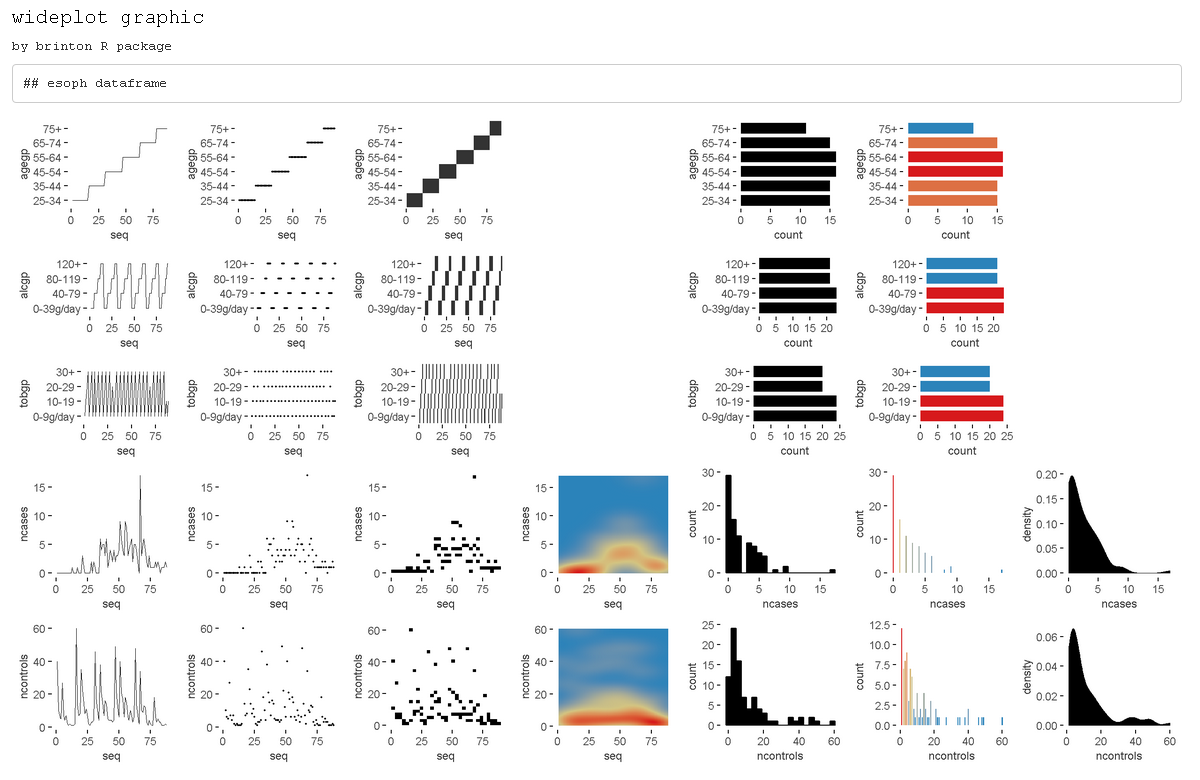
\includegraphics[width=0.95\linewidth]{figures/wideplot_esoph} \caption[Output of 'wideplot(esoph)']{Output of \texttt{wideplot(esoph)}. A grid of graphics in which each row corresponds to a variable in the dataset \texttt{esoph} and each column displays different available graphics.}\label{fig:wideplotesoph}
\end{figure}
\end{Schunk}

The \code{wideplot()} function creates html files, as side-effects, with
a graphical summary (See Figure \ref{fig:wideplotesoph}) of the
variables included in the dataset to which it has been applied. First it
groups the variables according to the following sequence: logical,
ordered, factor, character, datetime and numeric. Next, it creates a
multipanel graphic in html format, in which each variable of
the dataset is represented in a row of the grid, while each column
displays the different available graphics for each variable. We called
the resulting graphic type \emph{wideplot} because it shows a range of 
graphics for all of the columns of the dataset. The structure of the 
function, the arguments it permits and its default values are as follows:

\begin{Schunk}
\begin{Soutput}
#> wideplot(data, dataclass = NULL, logical = NULL, ordered = NULL,
#>   factor = NULL, character = NULL, datetime = NULL, numeric = NULL,
#>   group = NULL, ncol = 7, label = 'FALSE')
\end{Soutput}
\end{Schunk}

The only argument necessary to obtain a result is \code{data} that
expects a \code{data.frame} class object; \code{dataclass} selects and
sorts the types of variables to be shown; \code{ncol} filters the first
\emph{n} columns of the grid, between 3 and 7, which will be shown. The
fewer columns displayed, the larger the size of the resulting graphics,
a feature that is especially useful if the scale labels dwarf the
graphics area; \code{label} adds to the grid a vector below each group
of rows according to the variable type, with the names and order of the
graphics; \code{logical}, \code{ordered}, \code{factor},
\code{character}, \code{datetime} and \code{numeric} make it possible to
choose which graphics, from among the ones included by the specimen
(Sec. \ref{the-specimen}), appear in the grid and in what order, for
each variable type. Finally, \code{group} changes the selection of
graphics that are shown by default according to the criteria of Table 
\ref{tab:table1}.

If the order and graphic types to be shown for each variable type are
not specified and if the graphic types aren't filtered using the
argument \code{group}, then the default graphic will contain an
opinion-based selection of graphics for each variable type, organized
especially to facilitate comparison between graphics of the same row and
between graphics of the same column. The user can overwrite this
selection of graphics as needed, using the arguments \code{logical},
\code{ordered}, \code{factor}, \code{character}, \code{datetime} and
\code{numeric}.

\begin{table}[h!]
	\begin{tabular}{ll}\toprule
\textbf{group} & \textbf{graphic type}\\\midrule
\texttt{sequence} & includes the sequence in which the values are observed so that an axis\\
& develops this sequence. e.g. line graph, point-to-point graph\\
\texttt{scatter} & marks represent individual observations. e.g. point graph, stripe graph\\
\texttt{bin} & marks represent aggregated observations based on class intervals.\\
& e.g. histogram, bar graph\\
\texttt{model} & represents models based on observations. e.g. density plot, violin plot\\
\texttt{symbol} & represents models based on observations. and not only points, lines or areas\\
& e.g. box plot\\
\texttt{GOF} & represents the goodness of fit of some values with respect to a model\\
& e.g. qq plot \\
\texttt{random} & chosen at random\\
\bottomrule
	\end{tabular}
	\caption{Possible values for the \code{group} argument of the \code{wideplot()} function.}
	\label{tab:table1}
\end{table}

\hypertarget{the-longplot-function}{%
	\subsection{The longplot function}\label{the-longplot-function}}

To facilitate economy of calculation, the \code{wideplot()} function
presents a limited number of graphics in each row. If the user wants to
expand the range of suggested graphics for a given variable, he or she
should use the \code{longplot} function, which returns a grid with all
of the graphics considered by the package (See Figure
\ref{fig:longplotesophagegp}) for that variable. The structure of the
function is very simple \code{longplot(data, vars, label = TRUE)} and we
can easily check the outcome of applying this function to the variable
\code{alcgp} of the dataset \code{esoph}:


\begin{example}
  longplot(data = esoph, vars = "alcgp")
\end{example}

\vspace{-5pt}

\begin{Schunk}
	\begin{figure}[H]
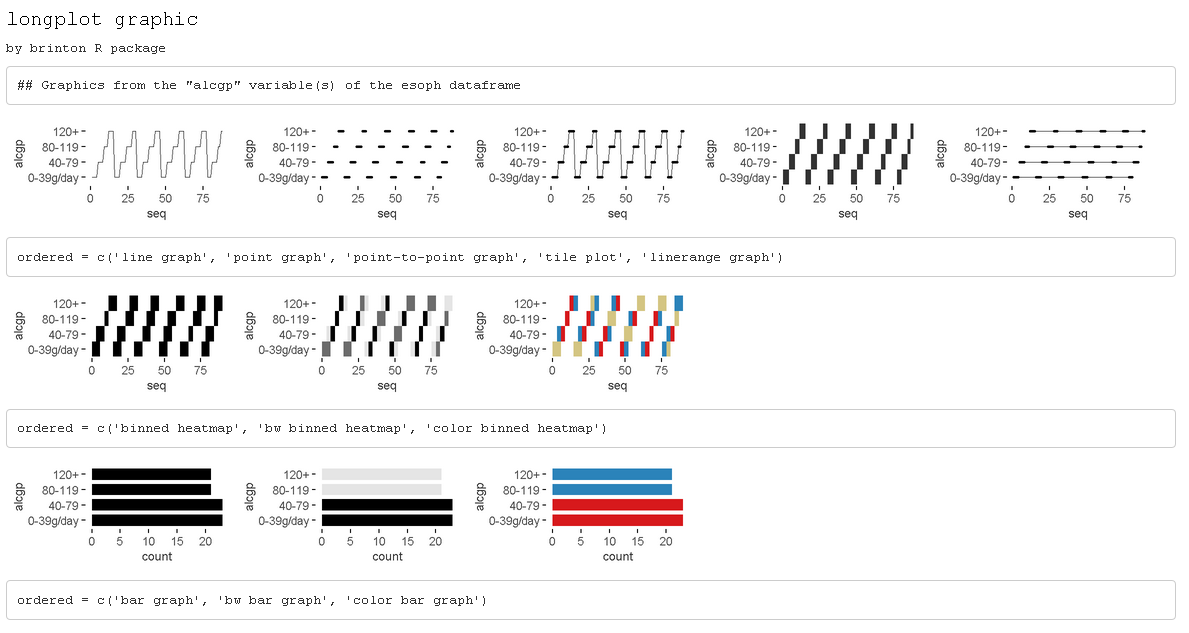
\includegraphics[width=0.95\linewidth]{figures/longplot_esoph_alcgp} \caption[Output of 'longplot(esoph, 'alcgp')']{Output of \texttt{longplot(esoph, 'alcgp')}. A grid of graphics where the variable \texttt{alcgp} in the dataset \texttt{esoph} is displayed for the full range of graphics considered by the package.}\label{fig:longplotesophagegp}
	\end{figure}
\end{Schunk}

We named the resulting graphic type \emph{longplot} because it shows the
full range of available graphics to represent the relationships among
the values of a limited selection of variables (although for now, in
this package we have only included graphics for a single variable).

The arguments of the function are \code{data}, which must be a
\code{data.frame} class object; \code{vars}, which requires the name of
a specific variable of the dataset; and \code{label}, which does not
have to be defined and which adds a vector below each row of the grid
indicating the name of each graphic. Unlike the grid of the
\code{wideplot} function, the grid of the \code{longplot} function does
not include parameters to limit the range of graphics to be presented.
We made this decision because the main advantage of this function is
precisely that it presents all of the graphic representations available
for a given variable. However, we do not rule out adding filters that
limit the number of graphics to be shown if this feature seems useful as
the catalog fills with graphics. Each graphic presented can be called
explicitly by name using the functions \code{wideplot()} and
\code{plotup()}, which is why the argument \code{label} has been set to
\code{TRUE} by default in this case.

The range of graphics that the \code{longplot()} function returns is
sorted so that in the rows we find different graphic types and in the
columns different variations of the same graphic type. This
organization, however, is not absolute and in some cases in order to
compress the results, we find different graphic types in the same row.

\hypertarget{the-plotup-function}{%
	\subsection{The plotup function}\label{the-plotup-function}}

The \code{plotup()} function has the following structure:
\code{plotup(data, vars, diagram, output = 'plots pane')}. By default,
this function returns an object belonging to class \code{gg} and 
\code{ggplot} whose graphic can be rendered in the plots pane of RStudio. 
This graphic is based on a variable from a given dataset and the name 
of the desired graphic, from among the names included by the specimen 
that we present in the next subsection. We can easily check the outcome 
of applying this function to produce a line graph from the variable 
\code{ncases} of the dataset \code{esoph} (See Figure 
\ref{fig:plotupesophncaseslinegraph}) :


\begin{example}
  plotup(data = esoph, vars = 'ncases', diagram = 'line graph', output = 'html')
\end{example}


\begin{Schunk}
	\begin{figure}[H]
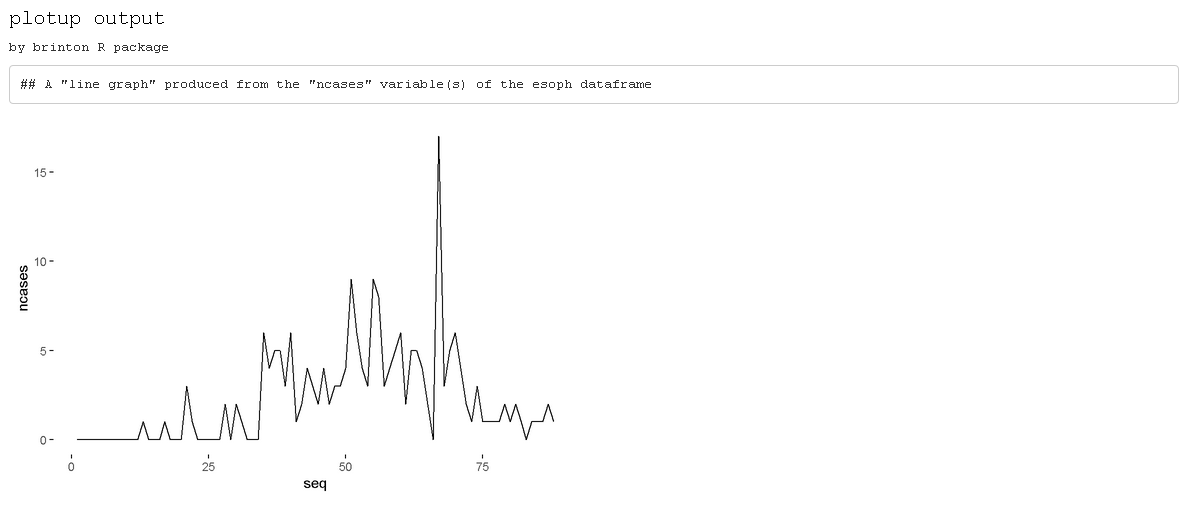
\includegraphics[width=0.90\linewidth]{figures/plotup_esoph_ncases_linegraph} \caption[Output of 'plotup(esoph, 'ncases', 'line graph', 'html')']{Output of \texttt{plotup(esoph, 'ncases', 'line graph')}. A line graph from the variable \texttt{ncases} in the dataset \texttt{esoph}.}\label{fig:plotupesophncaseslinegraph}
	\end{figure}
\end{Schunk}

This function requires three arguments: \code{data}, \code{vars} and
\code{diagram}. The fourth argument, \code{output}, is optional and has
the default value of \code{plots pane}. However, if is set to it
\code{html} or \code{console}, instead of returning a
\code{c("gg", "ggplot")} object, the function cause a side-effect:
either creating and displaying a temporary html file, or printing the
ggplot2 code to the console. This feature is especially useful to adapt
the default graphic to the specific needs and preferences of the user.

The \code{diagram} argument accepts any of the values admitted by the
\code{logical}, \code{ordered}, \code{factor}, \code{character},
\code{datetime} and \code{numeric} arguments of the \code{wideplot()}
function. These values coincide with the names of the graphics considered by the package and included in the specimen. The naming convention of these graphs is implicitly addressed in Section 4 ``Graphical degrees of freedom''.

\begin{example}
  plotup(data = esoph, vars = 'ncases', diagram = 'line graph', 
         output = 'console')
\end{example}

\begin{Schunk}
	\begin{Soutput}
#> ggplot(esoph, aes(x=seq_along(ncases), y=ncases)) +
#>   geom_line() +
#>   labs(x='seq') +
#>   theme_minimal() +
#>   theme(panel.grid = element_line(colour = NA),
#>     axis.ticks = element_line(color = 'black'))
	\end{Soutput}
\end{Schunk}



\hypertarget{the-specimen}{%
	\subsection{The specimen}\label{the-specimen}}

The documentation of the package includes the vignette ``1v specimen'',
which contains a specimen with images of all the graphic types for a
single variable, incorporated into the package according to the variable
type. These graphics serve as an example so that the user can rapidly
check whether a graphic has been incorporated, the type or types of
variable for which it has been incorporated, and the label with which it
has been identified. The suitability of a particular graphic will depend
on the datasets of interest and the variables of each particular user.
We have incorporated this specimen in its current version as
supplementary material.

\hypertarget{graphical-degrees-of-freedom}{%
	\section{Graphical degrees of
freedom}\label{graphical-degrees-of-freedom}}

The utility of this package is based on the fact that different
graphical representations of the same data make it possible not only to
observe different characteristics of the data, but also to show a
certain characteristic more effectively. For this reason, the graphics
considered by this package enjoy a large number of graphical degrees of
freedom. This makes it possible for the catalog to include both commonly
used graphics and graphics that have not yet been developed. The concept
of graphical degrees of freedom has been used by Benger and Hege
\citeyearpar{Benger2006} to refer to Bertin's visual variables
\citeyearpar[p.43]{Bertin1967} but with some modifications. Here we use
the concept in a broader sense, as detailed below.

\begin{itemize}
	\tightlist
	\item
	\textbf{Type of graphic}. The main degree of freedom of the graphics
	catalog is the graphic type. The different graphic types are not
	necessarily ones that differ greatly from each other. To the contrary,
	very similar graphics coexist because a high number of users prefer
	each of them. This is the case, for example, of the density plot and
	the violin plot shown in Figure \ref{fig:dg0}.
\end{itemize}


\begin{example}
  wideplot(data = esoph[5], 
           numeric = c('filled violin plot', 'filled density plot'))
\end{example}


\begin{Schunk}
	\begin{figure}[H]
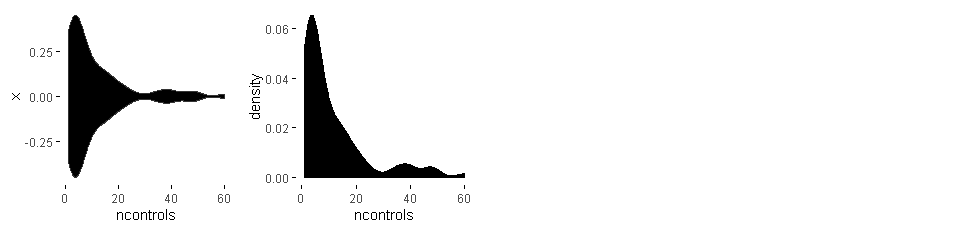
\includegraphics[width=1.0\linewidth]{figures/dg0-1} \caption[1st deg]{1st degree of freedom (type of graphic). Density and violin plots of variable \texttt{ncontrols} (in the dataset \texttt{esoph}).}\label{fig:dg0}
	\end{figure}
\end{Schunk}

\begin{itemize}
	\tightlist
	\item
	\textbf{Chromatic scales}. The same graphic can have different
	versions depending on the chromatic scale associated with a variable
	in the data or computed from it. We can see an example of this in the
	following figure \ref{fig:dg1}. Despite the fact that color can be
	broken down into the three visual variables of hue, saturation and
	value, for the purposes of this package we have only taken into
	account hue in the case of the color scale and value in the case of
	the grayscale, following Bertin's classification of visual variables
	\citeyearpar[p.43]{Bertin1967}.
\end{itemize}

\begin{example}
  wideplot(data = esoph[5], 
           numeric = c('histogram', 'bw histogram', 'color histogram'))
\end{example}


\begin{Schunk}
	\begin{figure}[H]
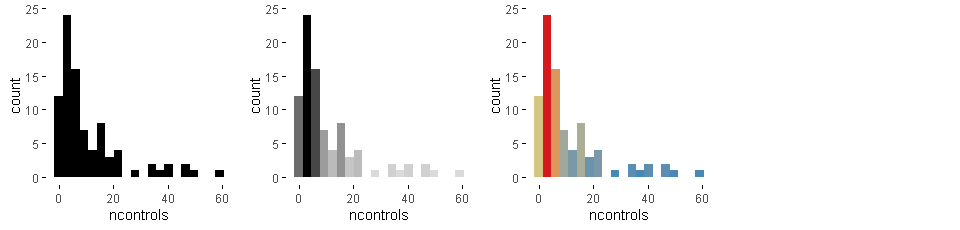
\includegraphics[width=1\linewidth]{figures/dg1-1} \caption[2nd deg]{2nd degree of freedom (chromatic scale). Plots of variable \texttt{ncontrols} (in the dataset \texttt{esoph}) with different chromatic scales.}\label{fig:dg1}
	\end{figure}
\end{Schunk}

\begin{itemize}
	\tightlist
	\item
	\textbf{Agreggation method: scattered or binned}. The same values can
	be represented such that each mark represents either a single value or
	an aggregate value. An example of this feature can be observed in
	Figure \ref{fig:dg2}.
\end{itemize}

\begin{example}
  wideplot(data = esoph[5], 
           numeric = c('stripe graph', 'binned stripe graph', 'bar graph', 
                       'histogram'))
\end{example}

\begin{Schunk}
	\begin{figure}[H]
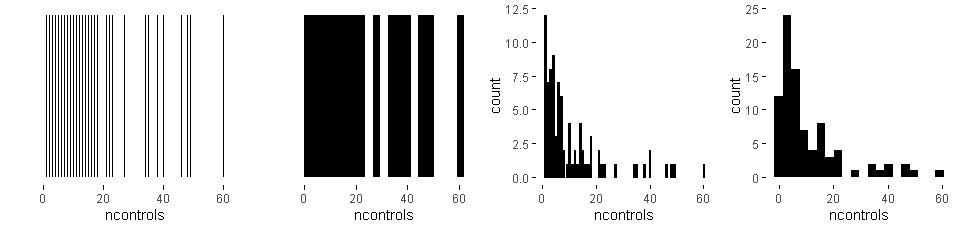
\includegraphics[width=1\linewidth]{figures/dg2-1} \caption[3rd deg]{3rd degree of freedom (aggregation method). Plots of variable \texttt{ncontrols} (in the dataset \texttt{esoph}) with single or aggregate values.}\label{fig:dg2}
	\end{figure}
\end{Schunk}

\begin{itemize}
	\tightlist
	\item
	\textbf{Nested panels}. One possibility (which has been little
	explored) is that of subdividing into different panels the cells of
	the multipanel graphic, to create systems of coordinates inside
	systems of coordinates. This solution is similar to the treemap. In
	the example in Figure \ref{fig:dg3}, the graphic on the right has
	three panels that can substitute the first three graphics.
\end{itemize}

\begin{example}
  wideplot(data = esoph[5], 
           numeric = c('violin plot', 'stripe graph', 'box plot', '3 uniaxial'))
\end{example}

\begin{Schunk}
	\begin{figure}[H]
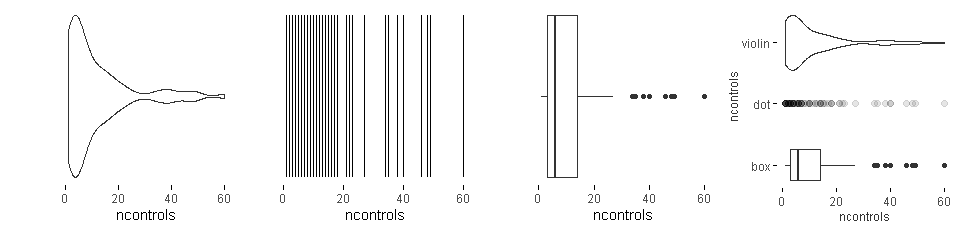
\includegraphics[width=1\linewidth]{figures/dg3-1} \caption[4th deg]{4th degree of freedom (nested panels). Plots of variable \texttt{ncontrols} (in the dataset \texttt{esoph}) with single and multiple panels (the first three ones and the last one respectively).}\label{fig:dg3}
	\end{figure}
\end{Schunk}

\begin{itemize}
	\tightlist
	\item
	\textbf{Shape}. The same information can be represented with marks of
	different shapes. This possibility is exemplified in Figure
	\ref{fig:dg4}, which compares two graphics with similar composition
	but different marks: circular or square.
\end{itemize}

\begin{example}
  wideplot(data = esoph[5], 
           numeric = c('color binned point graph', 'color binned heatmap'))
\end{example}


\begin{Schunk}
	\begin{figure}[H]
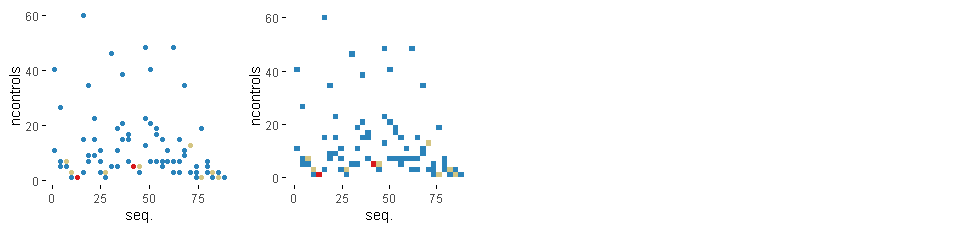
\includegraphics[width=1\linewidth]{figures/dg4-1} \caption[5th deg]{5th degree of freedom (shape). Plots of variable \texttt{ncontrols} (in the dataset \texttt{esoph}) with marks of different shapes.}\label{fig:dg4}
	\end{figure}
\end{Schunk}

\begin{itemize}
	\tightlist
	\item
	\textbf{Implantation}. The same values can be represented with marks
	of a different type of implantation, such as a point, a line, an area
	or a combination of these. For example, Figure \ref{fig:dg5} compares
	a point graph, a line graph, and a point-to-point graph.
\end{itemize}

\begin{example}
  wideplot(data = esoph[5], 
           numeric = c('point graph', 'line graph', 'point-to-point graph'))
\end{example}

\begin{Schunk}
	\begin{figure}[H]
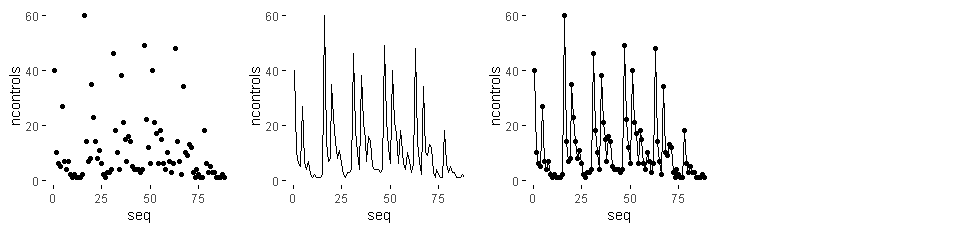
\includegraphics[width=1\linewidth]{figures/dg5-1} \caption[6th deg]{6th degree of freedom (implantation). Plots of variable \texttt{ncontrols} (in the dataset \texttt{esoph}) with marks of a different type of implantation.}\label{fig:dg5}
	\end{figure}
\end{Schunk}

\begin{itemize}
	\tightlist
	\item
	\textbf{Transition}. The transition or itinerary between two points
	can help reflect the discrete nature of the changes in the values
	observed. Figure \ref{fig:dg6} compares two line graphs with different
	transitions between points.
\end{itemize}

\begin{example}
  wideplot(data = esoph[5], 
           numeric = c('line graph', 'stepped line graph'))
\end{example}

\begin{Schunk}
	\begin{figure}[H]
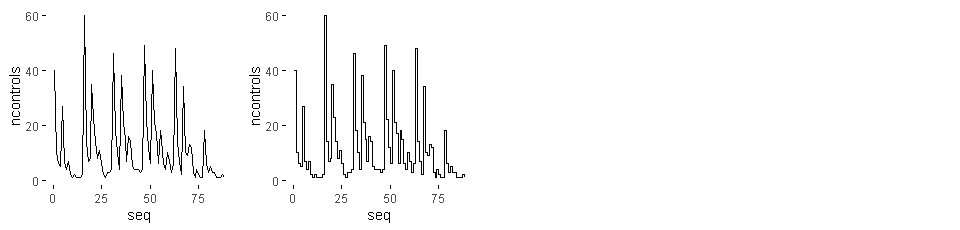
\includegraphics[width=1\linewidth]{figures/dg6-1} \caption[7th deg]{7th degree of freedom (transition). Plots of variable \texttt{ncontrols} (in the dataset \texttt{esoph}) with different transitions between points.}\label{fig:dg6}
	\end{figure}
\end{Schunk}

\begin{itemize}
	\tightlist
	\item
	\textbf{Collation}. The values of variables, especially those that
	aren't related to order, can be sorted according to different
	criteria. This package, as shown in Figure \ref{fig:dg7} uses three:
	the order of appearance in the sequence of observations, the frequency
	with which the values are observed and alphabetical order.
\end{itemize}

\begin{example}
  wideplot(data = data.frame('Region' = state.region),
           factor = c('tile plot',
                      'freq. reordered tile plot',
                      'alphab. reordered tile plot'))
\end{example}


\begin{Schunk}
	\begin{figure}[H]
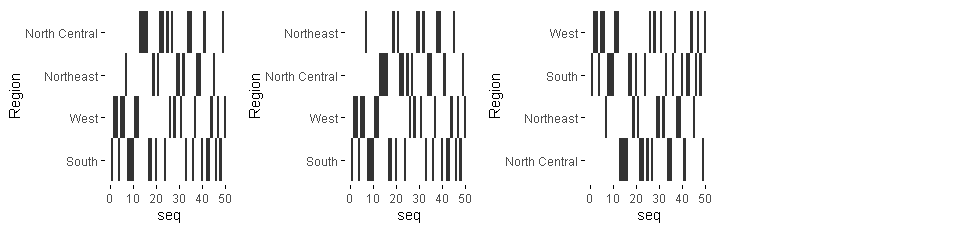
\includegraphics[width=1\linewidth]{figures/dg7-1} \caption[8th deg]{8th degree of freedom (collation). Plots of variable \texttt{Region} with the values sorted according to different criteria.}\label{fig:dg7}
	\end{figure}
\end{Schunk}

\begin{itemize}
	\tightlist
	\item
	\textbf{Superposition}. The final degree of freedom that we consider
	is the possibility of including graphics that superpose marks whose
	data source is the same but that have different degrees of
	transformation (see Figure \ref{fig:dg8}).
\end{itemize}

\begin{example}
  wideplot(data = esoph[5],  
           numeric = c('color point graph', 
                       'color point graph with trend line'))
\end{example}

\begin{Schunk}
	\begin{figure}[H]
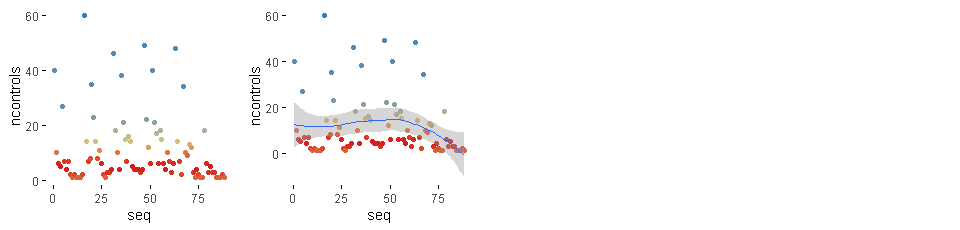
\includegraphics[width=1\linewidth]{figures/dg8-1} \caption[9th deg]{9th degree of freedom (superposition). Plots of variable \texttt{ncontrols} (in the dataset \texttt{esoph}) with and without the superposition of a trend line.}\label{fig:dg8}
	\end{figure}
\end{Schunk}

To construct the specimen we have ruled out some degrees of freedom, for
example, the group of imposition \citep[p.52]{Bertin1967} and the
permutation of spacial variables \citep[p.43]{Bertin1967}. In other
words, \pkg{brinton} package exclusively presents diagrams and not
networks or maps, nor does it show alternatives whose only difference is
that the \emph{x} and \emph{y} axes are switched.

\hypertarget{application-to-real-datasets}{%
	\section{Application to real
datasets}\label{application-to-real-datasets}}

The main application of a package for exploratory data analysis is to
help the user make sense of the data. This includes describing the
number and nature of the variables, the number of observations and
examples of the variables--this is precisely what the \code{str()}
function does. It also includes evaluating the validity and quality of
the data and the properties of the values found.

We can deduce the number of variables from the number of rows in the
grid of the wideplot graphic. The names of the variables are found in
each of the graphics that the catalog now contains. We can determine the
variables' nature--in terms of the measurement scale----by observing the
range of graphics selected and specifying the value \code{label = TRUE}
for the grids of wideplot and longplot graphics. We can discern the
number of observations by examining the graphics that include the
sequence of observations or, in the case of categorical variables, by
counting the categories and the number of observations for each one.
Wideplot graphics, in contrast to the textual summary of the
\code{str()} function, show examples not only of the first observations
but of all observations. To evaluate the validity of the data, we can
observe specific graphics that allow us to identify outliers, missing
values or discontinuity in the observations. The same goes for the
properties of the values found. There is a huge range of graphics, each
of which makes it possible to highlight different properties. Below we
list a series of tasks for which the functions included in \pkg{brinton}
are useful, and describe the process for carrying them out.

\hypertarget{identify-multi-column-sorting}{%
	\subsection{Identify multi-column
sorting}\label{identify-multi-column-sorting}}

Here we describe how to use the \code{wideplot()} function to determine
whether the observations of the dataset \code{aids} of the package
\CRANpkg{KMsurv} are sorted according to one of the variables. This dataset
has three variables, \code{infect} (infection time for AIDS in years),
\code{induct} (induction time for AIDS in years), and \code{adult}
(indicator of adult: 1=adult, 0=child). To accomplish the task, we first
install the package, then load it into memory and run the wideplot
function with its default output.

\begin{example}
  install.packages('KMsurv')
  data(aids, package = 'KMsurv')
  wideplot(data = aids, label = TRUE)
\end{example}


\begin{Schunk}
	\begin{figure}[H]
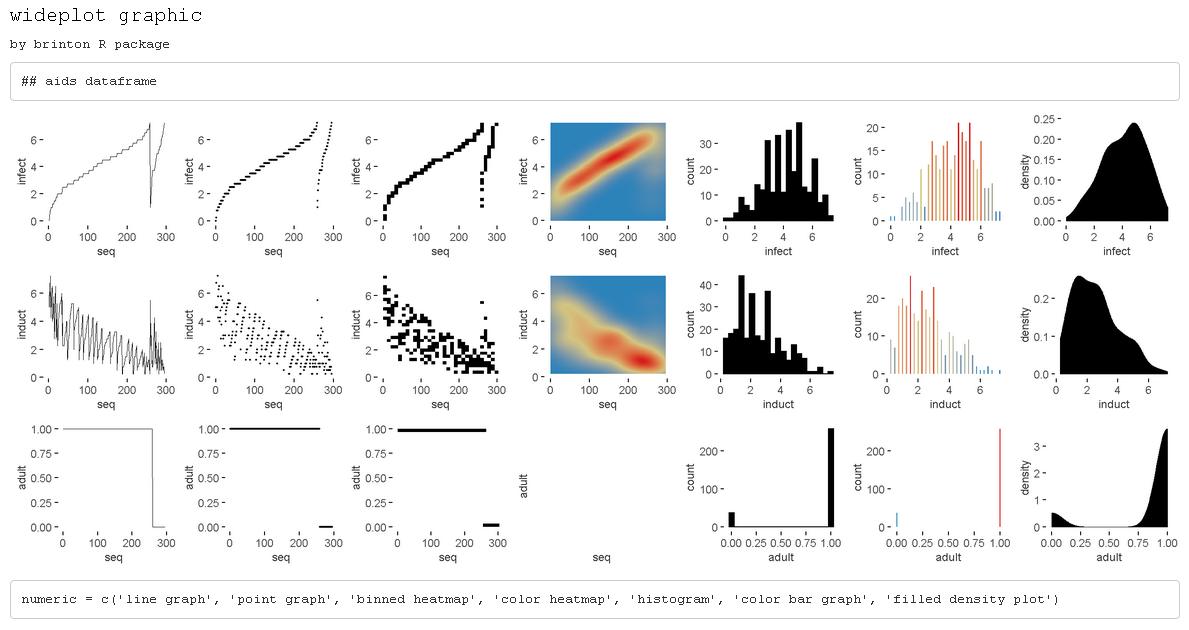
\includegraphics[width=0.9\linewidth]{figures/wideplot_aids0} \caption[Output of 'wideplot(aids, label = T)']{A grid of graphics generated by \texttt{wideplot(aids, label = T)}. Each row corresponds to a variable in the dataset \texttt{aids}. The line graph shows that the dataset is sorted first by the variable \texttt{adult} and then by the variable \texttt{infect}.}\label{fig:wideplotaids1}
	\end{figure}
\end{Schunk}

From the result in Figure \ref{fig:wideplotaids1}, we observe that the line graph is the one that best
shows that the dataset is sorted first by the variable \code{adult} and
then by the variable \code{infect}. To finish selecting the most
suitable graphic we can then execute the same function but limit the
graphic types such that only two variations of line graph are shown. We
can moreover limit the function so that it displays, for example, only
five columns, so that the graphics will be larger.

\begin{example}
  wideplot(data = aids, 
           numeric = c('line graph', 'stepped line graph'), ncol = 5)
\end{example}

\begin{Schunk}
	\begin{figure}[H]
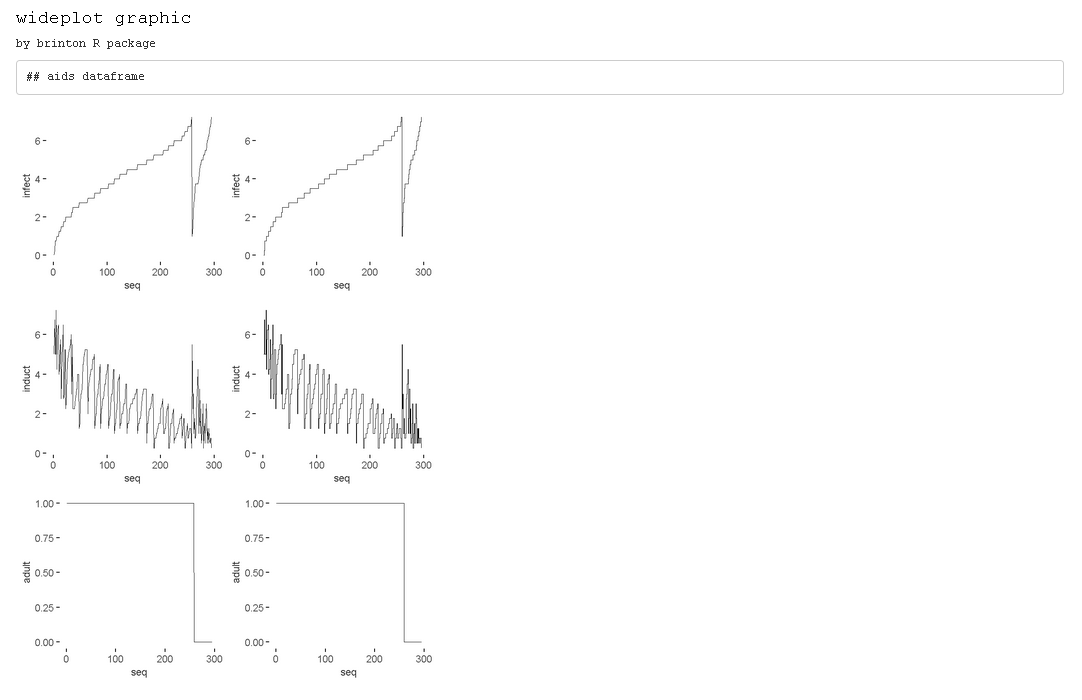
\includegraphics[width=0.9\linewidth]{figures/wideplot_aids} \caption[Output of 'wideplot(aids, numeric = c('line graph', 'stepped line graph'), ncol=5)']{A grid of graphics generated by \texttt{wideplot(aids, numeric = c('line graph', 'stepped line graph'), ncol=5)}. Each row corresponds to a variable in the dataset \texttt{aids}. Graphic types are limited to line and stepped line types.}\label{fig:wideplotaids2}
	\end{figure}
\end{Schunk}

The result is two variations of the line graph for each variable, in
which we can clearly see that the data set is sorted first by the
variable \code{adult} and then by the variable \code{infect}. In this
case, there may be equally valid arguments for using the graphics of the
first column as the graphics of the second column.

This same example also works for datasets with categorical variables,
such as the dataset MentalHealth of the package \CRANpkg{Stat2Data}. This
dataset consists of three variables: \code{Month} (month of the year);
\code{Moon} (relationship to full moon: \code{After}, \code{Before}, or
\code{During}); and \code{Admission} (number of emergency room
admissions). The first two variables are categorical and the third is
numerical. If we examine the line graph and also the tile plot for the
factor-type variables and the binned heatmap graphic for the numerical
variables, we can easily see that the dataset is sorted by the variable
\code{Moon} and then by the variable \code{Month} (see Figure
\ref{fig:wideplotmentalhealth}).

\begin{example}
  install.packages('Stat2Data')
  data(MentalHealth, package = 'Stat2Data')
  wideplot(data = MentalHealth, label = TRUE)
\end{example}

\begin{Schunk}
	\begin{figure}[H]
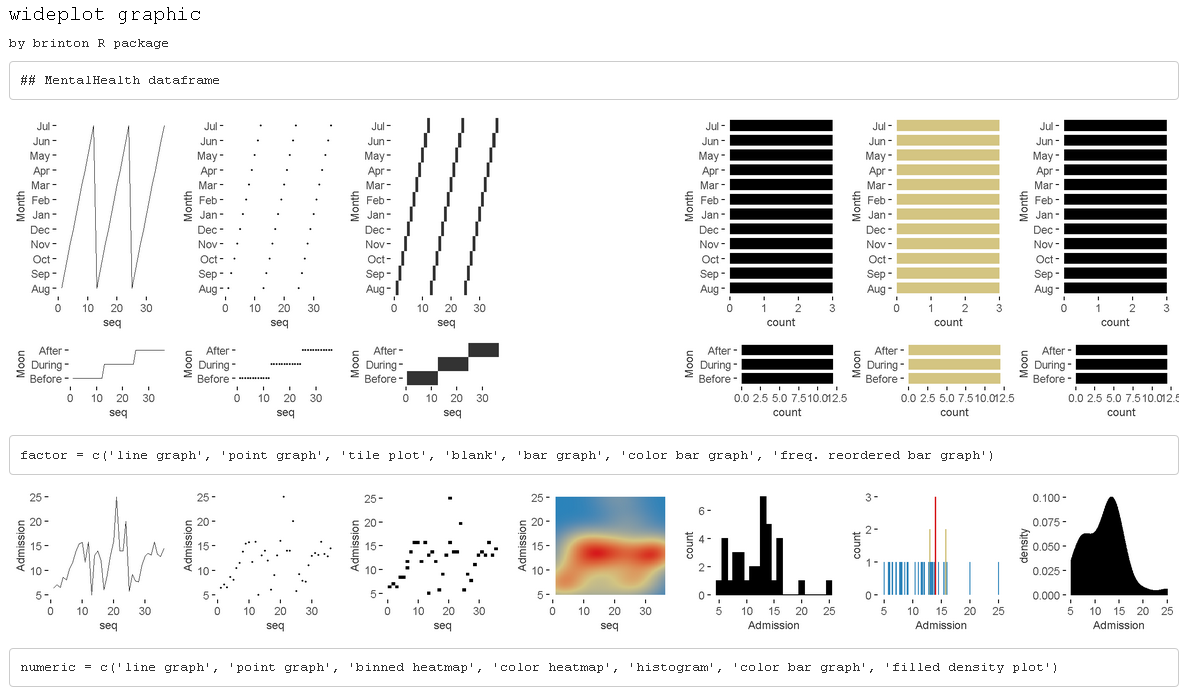
\includegraphics[width=0.8\linewidth]{figures/wideplot_MentalHealth0} \caption[Output of 'wideplot(MentalHealth, label = T)']{A grid of graphics generated by \texttt{wideplot(MentalHealth, label = T)}. Each row corresponds to a variable in the dataset \texttt{MentalHealth}. It is observed that the dataset is sorted by the variable \texttt{Moon} and then by the variable \texttt{Month}.}\label{fig:wideplotmentalhealth}
	\end{figure}
\end{Schunk}

\hypertarget{identify-variables-that-can-be-reclassified}{%
	\subsection{Identify variables that can be
reclassified}\label{identify-variables-that-can-be-reclassified}}

When loading a dataset it is important to check which assumptions the
function has made and which variables can be reclassified. We can see an
example of this in Figure \ref{fig:wideplotaids2}, which shows that the
variable \code{adult} of the dataset \code{aids} is better treated as a
logical-type variable than an integer. If we recode the variable type
more appropriately, when we apply the \code{wideplot()} function again,
the graphics also tend to be more appropriate. In Figure
\ref{fig:wideplotaids3} we see the result after the variable
\code{adult} is reclassified.

\begin{example}
  aids$adult <- as.logical(aids$adult)
  wideplot(data = aids)
\end{example}

\begin{Schunk}
	\begin{figure}[H]
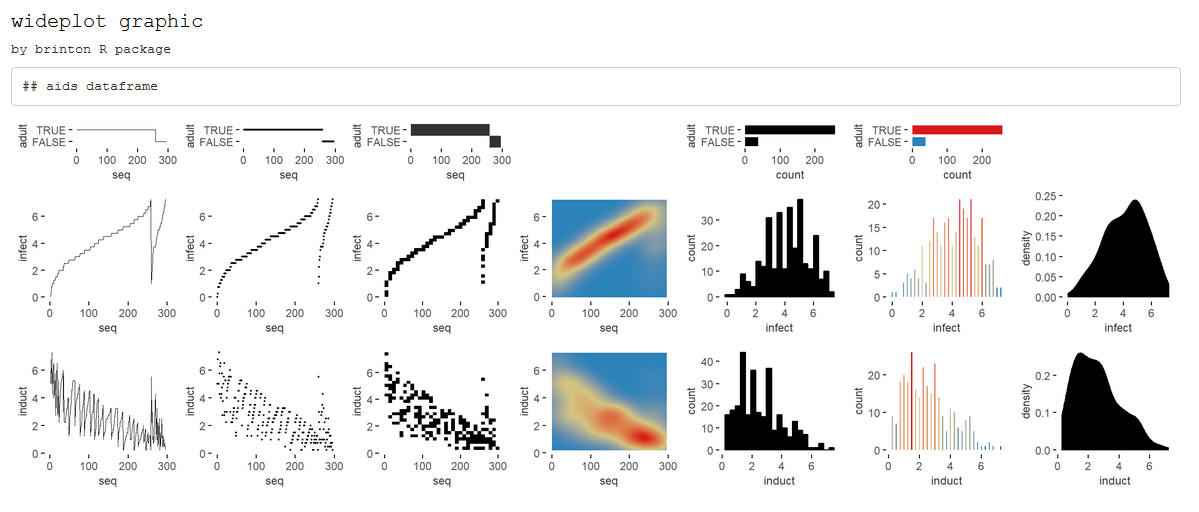
\includegraphics[width=0.8\linewidth]{figures/wideplot_aids2} \caption[Output of 'wideplot(aids)']{A grid of graphics generated by \texttt{wideplot(aids)}. Each row corresponds to a variable in the dataset \texttt{aids}. The variable \texttt{adult} has been reclassified from integer to logical in order to obtain more appropriate graphics.}\label{fig:wideplotaids3}
	\end{figure}
\end{Schunk}

\hypertarget{identify-key-variables}{%
	\subsection{Identify key variables}\label{identify-key-variables}}

The best way to identify key variables is by using complementary
graphics. Figure \ref{fig:wideplotazt} makes it possible, for example,
to identify rapidly the variable \code{patient} of the dataset
\code{azt} in the package \pkg{KMsurv}, as a key variable, given that it
assigns a sequential number to each record, each of which is observed a
single time. We can draw these two conclusions from the line graph and
the color bar graph.

\begin{example}
  data(azt, package = 'KMsurv')
  wideplot(data = azt, label = TRUE)
\end{example}

\begin{Schunk}
	\begin{figure}[H]
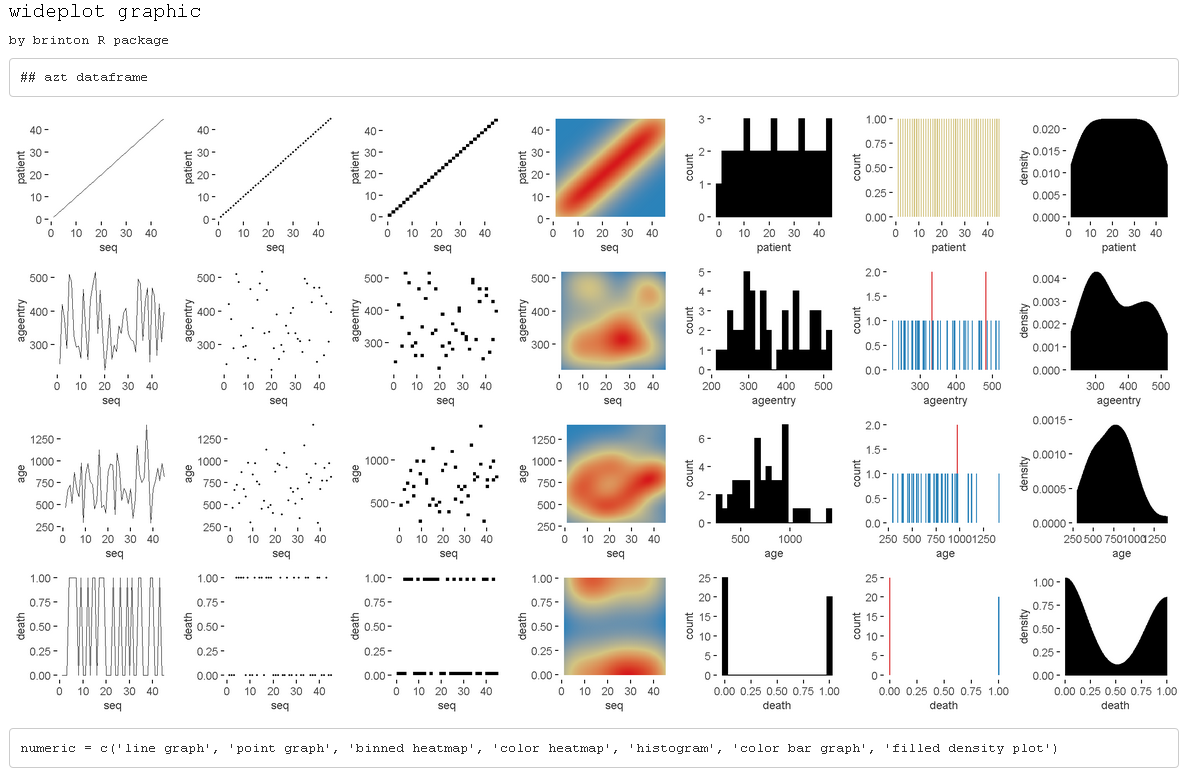
\includegraphics[width=0.9\linewidth]{figures/wideplot_azt} \caption[Output of 'wideplot(azt, label=TRUE)']{A grid of graphics generated by \texttt{wideplot(azt, label=TRUE)}. Each row corresponds to a variable in the dataset \texttt{azt}. The line graph and the color bar graph recognize the variable \texttt{patient} as a key variable that assigns a sequential number to each record.}\label{fig:wideplotazt}
	\end{figure}
\end{Schunk}

In the case of categorical key variables, the same line graph and color
bar graph would also help us to identify the key variable. Figure
\ref{fig:SpeciesArea} shows these two graphs for the factor-type
variable of the dataset \code{SpeciesArea} in the package
\pkg{Stat2Data}, which allow us to identify rapidly the variable
\code{Name} as a key variable.

\begin{example}
  data(SpeciesArea, package = 'Stat2Data')
  wideplot(data = SpeciesArea, dataclas = c('factor'), 
           factor = c('line graph', 'color bar graph'), ncol = 5)
\end{example}


\begin{Schunk}
	\begin{figure}[H]
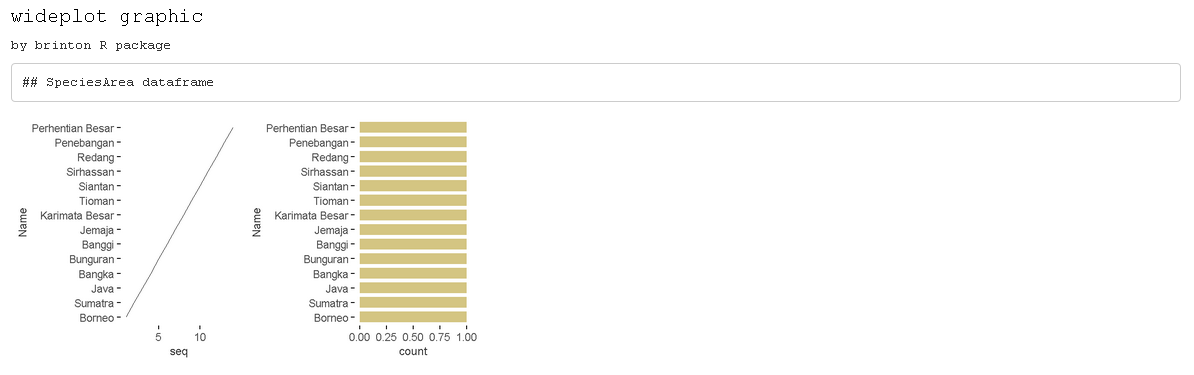
\includegraphics[width=0.8\linewidth]{figures/wideplot_SpeciesArea} \caption[Identification of key variables]{Line and color bar graphs of the factor-type variable \texttt{Name} (in the dataset \texttt{SpeciesArea}) produced by the function \texttt{wideplot()}. It is observed that the variable \texttt{Name} is a key variable since the values are not repeated and observed once.}\label{fig:SpeciesArea}
	\end{figure}
\end{Schunk}

\hypertarget{be-surprised-by-serendipity}{%
	\subsection{Be surprised by
serendipity}\label{be-surprised-by-serendipity}}

Next we describe isolated cases in which we are surprised by the values
that the data depict. We use the following procedure to locate
unexpected aspects of the data: first we obtain a general view of the
dataset using the function \code{wideplot()}; next we focus our
attention on one variable in particular and explore all of the
compatible graphics using the function \code{longplot()}; finally, we
use the function \code{plotup()} to obtain the graphic that best enables
us to identify, narrow down and communicate the aspect of the data that
we have found.

\begin{itemize}
	\tightlist
	\item
	The first example of an unexpected funding appears in the variable
	\code{experience} (years of potential work experience) of the dataset
	\code{HI} in the package \CRANpkg{Ecdat}. This dataset contains 22,272
	records of 13 variables that link health insurance policies to the
	weekly hours worked by the wives of the policyholders, while the
	variable \code{experience} refers to the years of potential work
	experience of the wives. If we look at the bar graph applied to this
	numerical variable (see Figure \ref{fig:HI_1}), we see that the
	frequency of the whole values is systematically greater than the
	frequency of the real non-whole values. This behavior could indicate
	that the variable can be informed with high precision and whoever
	informed the variable \code{experience} tended to round to the unit.
	Another possibility is that the dataset was constructed by joining two
	data sources with different degrees of precision\footnote{In the
following example we have decided to limit the number of records to
5,000 to reduce the calculation time and facilitate the reproduction
of these same examples.}
\end{itemize}

\begin{example}
  data(HI, package = 'Ecdat')
  HI_sam <- HI[sample(nrow(HI), 5000), ]
  wideplot(data = HI_sam)                      # Output not reproduced here
  longplot(data = HI_sam, vars = 'experience') # Output not reproduced here
  plotup(data = HI_sam, vars = 'experience', diagram = 'bar graph')
\end{example}

\begin{Schunk}
	\begin{figure}[H]
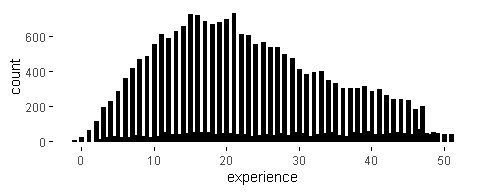
\includegraphics[width=0.5\linewidth]{figures/HI_1-1} \caption[Identification of rounded values]{Bar plot of the variable \texttt{experience} (in the dataset \texttt{HI}) produced by the function \texttt{plotup()}. It is observed that the frequency of the whole values is systematically greater than the frequency of the real non-whole values.}\label{fig:HI_1}
	\end{figure}
\end{Schunk}

\begin{itemize}
	\tightlist
	\item
	In the same dataset we can see that we could reach mistaken
	conclusions about the distribution of the variable \code{husby}
	(husband's income in thousands of dollars) if we only looked at a
	histogram. As we can see in Figure \ref{fig:HI_2}, the distribution,
	and in particular the value zero, acquires a different value if we
	compare the histogram (left) with another graphic that isn't as
	common for numerical variables: the bar graph (right), which shows the
	count of unique values. The bar graph makes it possible to clearly
	differentiate two groups: the informants whose husbands have no income
	and the informants whose husbands do have income (and to whom,
	therefore, it makes more sense to ask approximate income).
\end{itemize}

\begin{example}
  library(patchwork)
  plotup(HI_sam, 'husby', 'histogram') + plotup(HI_sam, 'husby', 'bar graph')
\end{example}

\begin{Schunk}
	\begin{figure}[H]
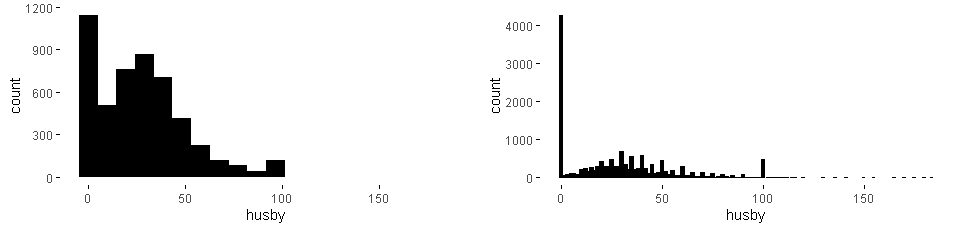
\includegraphics[width=1\linewidth]{figures/HI_2-1} \caption[Identification of values with a special meaning]{Histogram (left) and bar plot (right) of the variable \texttt{husby} (in the dataset \texttt{HI\_sam}) produced by the function \texttt{plotup()}. The bar plot makes it possible to identify the zero as a value with a special meaning.}\label{fig:HI_2}
	\end{figure}
\end{Schunk}

\hypertarget{combine-graphics-that-best-explains-a-specific-data-characteristic}{%
	\subsection{Combine graphics that best explains a specific data
characteristic}\label{combine-graphics-that-best-explains-a-specific-data-characteristic}}

Just as multipanel graphics make it possible to reveal different aspects
of the data, it can also be helpful to use a selection of graphics to
present a certain characteristic of the data. Next, we show an example
of how \pkg{brinton} package can help us improve the default graphics in
order to combine them later to show a particular feature.

\begin{itemize}
	\tightlist
	\item
	A recurring problem when we deal with datasets with many records is
	that when marks overlap, we cannot correctly interpret the set of
	observations. The presentation of multiple graphics to represent the
	same values enables us to identify these overlaps and improve the
	representation that the package shows by default. For example, in
	Figure \ref{fig:HI_3} we can see how the point graph for the same
	variable \code{husby} is unclear because the marks overlap.
\end{itemize}

\begin{example}
  plotup(data = HI_sam, vars = 'husby', diagram = 'point graph')
\end{example}

\begin{Schunk}
	\begin{figure}[H]
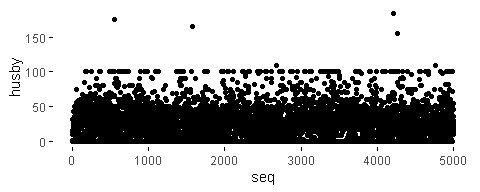
\includegraphics[width=0.6\linewidth]{figures/HI_3-1} \caption[To be honest, a very improvable point graph]{Point plot of the variable \texttt{husby} (in the dataset \texttt{HI\_sam}) produced by the function \texttt{plotup()}. The point plot does not identify the zero as a value with a special meaning because the marks overlap.}\label{fig:HI_3}
	\end{figure}
\end{Schunk}

\begin{itemize}
	\tightlist
	\item
	We do not have to accept the default result. Rather we can retrieve
	the package's \pkg{ggplot2} function using the argument
	\code{output = 'console'} and then improve it:
\end{itemize}

\begin{example}
  plotup(data = HI_sam, vars = 'husby', diagram = 'point graph', 
  output = 'console')
\end{example}

\begin{Schunk}
	\begin{Soutput}
#> ggplot(HI_sam, aes(x=seq_along(husby), y=husby)) +
#>   geom_point() +
#>   labs(x='seq') +
#>   theme_minimal() +
#>   theme(panel.grid = element_line(colour = NA),
#>     axis.ticks = element_line(color = 'black'))
	\end{Soutput}
\end{Schunk}

\begin{itemize}
	\tightlist
	\item
	In this case we can, for example, improve the graphic by reducing the
	size of the points and adding an alpha channel (see Figure
	\ref{fig:HI_4}).
\end{itemize}

\begin{example}
  newpointgraph <- ggplot(HI_sam, aes(x=seq_along(husby), y=husby)) +
  geom_point(size = 0.3, alpha = 0.15) + 
  labs(x='seq') +
  theme_minimal() +
  theme(panel.grid = element_line(colour = NA), 
  axis.ticks = element_line(color = 'black'))

  newpointgraph
\end{example}

\begin{Schunk}
	\begin{figure}[H]
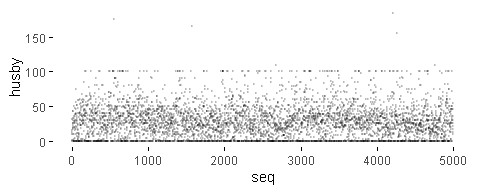
\includegraphics[width=0.6\linewidth]{figures/HI_4-1} \caption[Improved output]{New point plot of the variable \texttt{husby} (in the dataset \texttt{HI\_sam}) produced by the functions \texttt{plotup()} and \texttt{ggplot()}. Now the point plot makes it possible to identify the zero as a value with a special meaning.}\label{fig:HI_4}
	\end{figure}
\end{Schunk}

\begin{itemize}
	\tightlist
	\item
	One option for this graphic that isn't affected by the overlapping of
	marks is the heatmap, and yet another is the bar graph that represents
	the frequency with which the unique values are observed. Combining the
	three graphics helps to highlight different aspects in order to make
	it easier to understand the data. Figure \ref{fig:lastone} shows how
	to combine the three graphics. Note that the bar graph has been
	rotated 90 degrees to become a marginal plot, following the grammar
	implemented in \pkg{ggplot2}, to facilitate the correspondence between
	individual observations, the density that can be deduced from them,
	and the frequency of unique values. Also, the axis labels have been
	adjusted to avoid unnecessary repetition.
\end{itemize}

\begin{example}
  newpointgraph + labs(y = "husband's income * 1000$") +
  plotup(data = HI_sam, vars = 'husby', diagram = 'color heatmap') +
  labs(y = '') +
  plotup(data = HI_sam, vars = 'husby', diagram = 'bar graph') +
  labs(x = '') + coord_flip()
\end{example}
	
\begin{Schunk}
\begin{figure}[H]
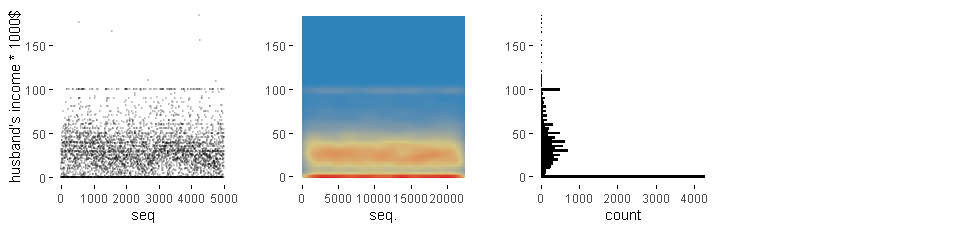
\includegraphics[width=1\linewidth]{figures/lastone-1} \caption[Multipanel graphic as a composition of plotup outputs]{Multipanel graphic as a composition of three plots of the variable \texttt{husby} (in the dataset \texttt{HI\_sam}). The source of each plot is the function \texttt{plotup()}. Combining the three plots helps to highlight different aspects of the distribution of the variable \texttt{husby}.}\label{fig:lastone}
\end{figure}
\end{Schunk}

The resulting multipanel graphic shows that throughout the dataset, the
revenue distribution remains essentially constant, highlighting the
number of husbands without income and rounding the reported values to
nice numbers such as 25, 30, 40, 50 and 100--although in reality, the
value that draws a horizontal line around 100 is, surprisingly, 99,999.
And here we have another mystery to solve.

\hypertarget{conclusions}{%
	\section{Conclusions}\label{conclusions}}

We have introduced \pkg{brinton} package, a graphical EDA tool designed
to facilitate the presentation, selection and editing of statistical
graphics built on \pkg{ggplot2}. This package maximizes the
deterministic strategy of graphic selection by presenting a range of
graphics that a user can choose by name, automating the construction of
graphics and even allowing the user to recover the underlying
\pkg{ggplot2} function in order to adapt the graphics as necessary. This
package makes it easier for a user to become familiar with a dataset and
generate hypotheses based on it.

This is a project in progress and new software implementations are being 
updated and released.  We plan to create a fuller catalog that will include 
graphics that can combine up to three variables, improve the aesthetics of 
the default graphics and add new functions for autoGEDA.

\hypertarget{acknowledgements}{%
	\section{Acknowledgements}\label{acknowledgements}}

We thank Michael Friendly and Pedro Valero-Mora for corresponding with
AUTHOR 1 about the package \pkg{cowplot}, which inspired the
\texttt{wideplot()} function that forms the core of this package. We 
acknowledge Susan Frekko for translating so accurately the manuscript from 
Catalan.

\bibliography{millan}


\address{%
	Pere Millán-Martínez\\
	Servei Català de Trànsit\\
	Carrer Diputació, 355 08009 Barcelona, Spain\\
	Research Group on Methodology, Methods, Models and Outcomes of Health and Social Sciences ($M_{3}O$)\\
	Faculty of Health and Welfare Sciences\\
	Universitat de Vic - UCC\\
	Sagrada Família, 7 08500 Vic, Spain\\
	ORCID: 0000-0003-0879-9358\\
}
\href{mailto:info@sciencegraph.org}{\nolinkurl{info@sciencegraph.org}}

\address{%
	Ramon Oller\\
	Data Analysis and Modeling Research Group\\
	Departament d'Economia i Empresa\\
	Universitat de Vic - UCC\\
	Sagrada Família 7, 08500 Vic, Spain\\
	ORCID: 0000-0002-4333-0021\\
}
\href{mailto:ramon.oller@uvic.cat}{\nolinkurl{ramon.oller@uvic.cat}}
